\documentclass[11pt,a4paper]{article}
%--------------------------------------------------
%Packages bases
\usepackage{lmodern}
\usepackage[spanish]{babel}
\usepackage[utf8]{inputenc}
\usepackage{array}
\usepackage{ifthen}
\usepackage{transparent}
\usepackage{eso-pic}
\usepackage{multirow}
\usepackage{afterpage}
\usepackage{amsfonts}
\usepackage{amssymb}
\usepackage{amsthm}
\usepackage{float}
\usepackage{ifthen}
\usepackage{framed}
\usepackage{xspace}
\usepackage{multicol}
\usepackage{enumitem}
\usepackage{color}
\usepackage{titlesec}
\usepackage{ifthen}


%----------------------------------------
%design
\usepackage{amsmath,tikz}
\usepackage{verbatim}
\usetikzlibrary{shapes.geometric}
\usetikzlibrary{arrows}

%----------------------------------------
%color
\usepackage{transparent}
\usepackage{colortbl}
\definecolor{darkred}{rgb}{.7,0.03,0.22}
\definecolor{red_tab}{rgb}{0.96,0.88,0.86}
\definecolor{darkblue}{HTML}{0000CC}
\definecolor{vdarkblue}{HTML}{000066}
\definecolor{texte}{HTML}{660099}
\definecolor{comt}{HTML}{009933}
%-----------------------------------------


%------------------------------------------
%counters
\newcounter{step}
\newcounter{substep}
\setcounter{step}{0}
\setcounter{substep}{0}
%------------------------------------------

\usepackage{tabularx}
\usepackage{makecell}


\newcolumntype{R}[1]{>{\raggedleft\arraybackslash }p{#1}}
\newcolumntype{L}[1]{>{\raggedright\arraybackslash }p{#1}}
\newcolumntype{C}[1]{>{\centering\arraybackslash }p{#1}}

\usepackage{wasysym}


\usepackage{ifluatex}
\ifluatex
\usepackage{fontspec}
\usepackage{polyglossia}
\setdefaultlanguage{french}
\else
\usepackage[utf8]{inputenc}
\usepackage[T1]{fontenc}
\usepackage{babel}


%-----------------------------------------
%format page
\usepackage[a4paper,left=2cm,right=1cm,top=0.5cm,bottom=1cm,headheight=0cm, headsep=0cm, footskip=0cm,includefoot,includehead]{geometry}

%----------------------------------------
%footnote and header number
\usepackage{fancyhdr}
\usepackage[pages=all]{background}
\pagestyle{fancy}
\renewcommand{\headrulewidth}{0pt}
\fancyhf {} % clear all headers and footers

% Header is used to include the page background
\backgroundsetup{
scale=1,
color=black,
opacity=1,
angle=0,
contents={%
  
\includegraphics[width=\paperwidth,height=\paperheight]{images/paper.jpg}
  }%
}

%-----------------------------------------
%Hyperlink
\usepackage[colorlinks, bookmarks, linkcolor=black, citecolor=black, urlcolor=blue]{hyperref}

%-----------------------------------------
%Set Monospace font
% \usepackage{everysel}
%     \renewcommand*\familydefault{\ttdefault}
%     \EverySelectfont{%
%     \fontdimen2\font=0.4em  % interword space
%     \fontdimen3\font=0.2em  % interword stretch
%     \fontdimen4\font=0.1em  % interword shrink
%     \fontdimen7\font=0.1em  % extra space
%     \hyphenchar\font=`\-    % to allow hyphenation
% }
%-----------------------------------------
%Configurations
\newcommand{\Style}[1]{
\ifthenelse{#1=1}{\makeatletter
\newcommand{\PrepTime}[1]{\def\@PrepTime{#1\xspace}
\def\PrepTimeb{#1}}
\newcommand{\CookingTime}[1]{\def\@CookingTime{#1\xspace}}
\newcommand{\background}[1]{%
\AddToShipoutPictureBG{\AtPageLowerLeft{\transparent{0.1}\includegraphics[width=\paperwidth,height=\paperheight]{#1}}}
}
\newcommand{\CookingTempe}[1]{%
\ifnum0=#1\relax
   \def\@CookingTempe{} 
\else
  \def\@CookingTempe{-- #1$^{\circ}$} 
\fi
}

\newcommand{\TypeCooking}[1]{\def\@TypeCooking{#1}}
\newcommand{\NPerson}[1]{\def\@NbPerson{#1\xspace}}
\newcommand{\Image}[2]{\def\@ImageDim{#1} \def\@ImagePath{#2}}
\def\maketitle{%

\vspace*{0.05cm}
\begin{center}
{\Huge \@title}
\end{center}
}

\newenvironment{ingredient}
  {\noindent\begingroup\edef\x{\endgroup\noexpand}\x
  \maketitle
  
  \begin{footnotesize}\noindent\setlength\arrayrulewidth{2pt}\begin{tabular}{|L{0.62\linewidth}|L{0.33\linewidth}|}\hline\vspace{-0.21cm}\underline{\textbf{{\normalsize Ingredients (\@NbPerson persons):}}} &\\
  \begin{minipage}{\linewidth}
  \vspace{0.2cm}
  }
  {\vspace{-0.2cm}
  \end{minipage}& \vspace{-1.8cm}Preparation time: \begin{tikzpicture}
  \pgfmathsetmacro{\timeor}{\PrepTimeb}
  \ifthenelse{\timeor>60}{
  \pgfmathsetmacro{\timeorb}{90-(\PrepTimeb-60)/60*360}
  \fill[orange] (0,0.55) arc(90:-270:0.55)      -- ++(-270:-0.55)
  arc(-270:0:0)    -- cycle;
  \fill[red] (0,0.55) arc(90:\timeorb:0.55)      -- ++(\timeorb:-0.55)
  arc(\timeorb:0:0)    -- cycle;
  }{
  \pgfmathsetmacro{\timeorb}{90-(\PrepTimeb)/60*360}
  \fill[green] (0,0.55) arc(90:\timeorb:0.55)      -- ++(\timeorb:-0.55)
  arc(\timeorb:0:0)    -- cycle;
  }
  \node[fill=white,inner sep=0pt] at (0,0) {{\tiny \PrepTimeb~min}};
  \fill[black!50,even odd rule] (0,0) circle(0.65) circle(0.6);
  \fill[black!50,even odd rule] (0,0.5) circle(0.05);
  \fill[black!50,even odd rule] (0.5,0) circle(0.05);
  \fill[black!50,even odd rule] (0,-0.5) circle(0.05);
  \fill[black!50,even odd rule] (-0.5,0) circle(0.05);
  \end{tikzpicture} \par
  \vspace{0.2cm} Cooking: \@CookingTime min \@CookingTempe

  
   \par \vspace{0.2cm} Cooking Type: \@TypeCooking \\\hline\end{tabular}\vspace{0.5cm} \end{footnotesize}}


\newenvironment{main}
  {\begin{multicols}{2}
  \begin{itemize}[label=$$]
  }
  {\end{itemize}\end{multicols}}
  
\newenvironment{subingredient}[1]
{\vspace{-0.3cm}\hspace{0.5cm}\underline{#1:}
\vspace{-0.3cm}\begin{multicols}{2}
\begin{itemize}[label=$$]
}
{\end{itemize}\end{multicols}}


\newenvironment{recipe}
{
}
{}
\makeatother

%-----------------------------------------
%New environments

\newenvironment{notes}
{\vfill\def\FrameCommand{\fboxsep=\FrameSep\fbox}%
\MakeFramed {\advance\hsize-\width \FrameRestore}
\noindent\underline{\textbf{Notes and tips:}}%

\vspace{0.25cm}
\noindent\hspace{-0.15cm}}
{\vspace{2.5cm}\endMakeFramed}
  
  
\newcommand{\step}[1]{\ifthenelse{\value{step}=0}{\noindent{\large \underline{\textbf{Preparation:}}}\vspace{0.3cm}

}{}
\noindent\stepcounter{step}\setcounter{substep}{0}\the\value{step}. #1\vspace{0.3cm}

} 

\newcommand{\substep}[2][1]{\ifthenelse{\value{substep}=0}{\noindent\stepcounter{step}\the\value{step}. \underline{\textbf{#1:}}\vspace{0.3cm}

}{}
\hspace{0.3cm}\begin{minipage}{0.948\textwidth}
\noindent\stepcounter{substep}\roman{substep}. #2\vspace{0.5cm}
\end{minipage}

}   }{}
\ifthenelse{#1=2}{\makeatletter
\newcommand{\PrepTime}[1]{\def\@PrepTime{#1\xspace}
\def\PrepTimeb{#1}}
\newcommand{\CookingTime}[1]{\def\@CookingTime{#1\xspace}}
\newcommand{\background}[1]{%
\AddToShipoutPictureBG{\AtPageLowerLeft{\transparent{0.1}\includegraphics[width=\paperwidth,height=\paperheight]{#1}}}
}
\newcommand{\CookingTempe}[1]{%
\ifnum0=#1\relax
   \def\@CookingTempe{} 
\else
  \def\@CookingTempe{-- #1$^{\circ}$} 
\fi
}

\newcommand{\TypeCooking}[1]{\def\@TypeCooking{#1}}
\newcommand{\NPerson}[1]{\def\@NbPerson{#1\xspace}}
\newcommand{\Image}[2]{\def\@ImageDim{#1} \def\@ImagePath{#2}}
\def\maketitle{%

\vspace*{0.05cm}
\begin{center}
{\Huge \@title}
\end{center}
}

\newenvironment{ingredient}
  {\noindent\begingroup\edef\x{\endgroup\noexpand}\x
  \maketitle
  
  \begin{footnotesize}\noindent\setlength\arrayrulewidth{2pt}\begin{tabular}{|L{0.62\linewidth}|L{0.33\linewidth}|}\hline\vspace{-0.21cm}\underline{\textbf{{\normalsize Ingredientes (\@NbPerson personas):}}} &\\
  \begin{minipage}{\linewidth}
  \vspace{0.2cm}
  }
  {\vspace{-0.2cm}
  \end{minipage}& \vspace{-1.8cm}Tiempo de preparación: \begin{tikzpicture}
  \pgfmathsetmacro{\timeor}{\PrepTimeb}
  \ifthenelse{\timeor>60}{
  \pgfmathsetmacro{\timeorb}{90-(\PrepTimeb-60)/60*360}
  \fill[orange] (0,0.55) arc(90:-270:0.55)      -- ++(-270:-0.55)
  arc(-270:0:0)    -- cycle;
  \fill[red] (0,0.55) arc(90:\timeorb:0.55)      -- ++(\timeorb:-0.55)
  arc(\timeorb:0:0)    -- cycle;
  }{
  \pgfmathsetmacro{\timeorb}{90-(\PrepTimeb)/60*360}
  \fill[green] (0,0.55) arc(90:\timeorb:0.55)      -- ++(\timeorb:-0.55)
  arc(\timeorb:0:0)    -- cycle;
  }
  \node[fill=white,inner sep=0pt] at (0,0) {{\tiny \PrepTimeb~min}};
  \fill[black!50,even odd rule] (0,0) circle(0.65) circle(0.6);
  \fill[black!50,even odd rule] (0,0.5) circle(0.05);
  \fill[black!50,even odd rule] (0.5,0) circle(0.05);
  \fill[black!50,even odd rule] (0,-0.5) circle(0.05);
  \fill[black!50,even odd rule] (-0.5,0) circle(0.05);
  \end{tikzpicture} \par
  \vspace{0.2cm} Cocción: \@CookingTime min \@CookingTempe

   \par \vspace{0.2cm} Tipo de cocción: \@TypeCooking \\\hline\end{tabular}\vspace{0.5cm} \end{footnotesize}}


\newenvironment{main}
  {\begin{multicols}{2}
  \begin{itemize}[label=$$]
  }
  {\end{itemize}\end{multicols}}
  
\newenvironment{subingredient}[1]
{\vspace{-0.3cm}\hspace{0.5cm}\underline{#1:}
\vspace{-0.3cm}\begin{multicols}{2}
\begin{itemize}[label=$$]
}
{\end{itemize}\end{multicols}}


\newenvironment{recipe}
{
}
{}
\makeatother

%-----------------------------------------
%New environments

\newenvironment{notes}
{\vfill\def\FrameCommand{\fboxsep=\FrameSep\fbox}%
\MakeFramed {\advance\hsize-\width \FrameRestore}
\noindent\underline{\textbf{Notas y tips:}}%

\vspace{0.25cm}
\noindent\hspace{-0.15cm}}
{\vspace{1cm}\endMakeFramed}
  
  
\newcommand{\step}[1]{\ifthenelse{\value{step}=0}{\noindent{\large \underline{\textbf{Preparación:}}}\vspace{0.3cm}

}{}
\noindent\stepcounter{step}\setcounter{substep}{0}\the\value{step}. #1\vspace{0.3cm}

} 

\newcommand{\substep}[2][1]{\ifthenelse{\value{substep}=0}{\noindent\stepcounter{step}\the\value{step}. \underline{\textbf{#1:}}\vspace{0.3cm}

}{}
\hspace{0.3cm}\begin{minipage}{0.948\textwidth}
\noindent\stepcounter{substep}\roman{substep}. #2\vspace{0.5cm}
\end{minipage}

}   }{}}



\makeatletter

%% Define the var grade
\def\grade#1{\def\@grade{#1}}
\def\gradex{\@grade}

%% Define the var subject
\def\subject#1{\def\@subject{#1}}
\def\subjectx{\@subject}

%% Define the var activity
\def\activity#1{\def\@activity{#1}}
\def\activityx{\@activity}

%% Define the var number of description
\def\description#1{\def\@description{#1}}
\def\descriptionx{\@description}

%% Define the var title
\def\title#1{\def\@title{#1}}
\def\titlex{\@title}

%% Define the var subtitle
\def\subtitle#1{\def\@subtitle{#1}}
\def\subtitlex{\@subtitle}

%% Define the var image
% Structure: \image[scale=0.5]{example-image-a}
\newcommand*{\image}[2][scale=0.5]{%
  \gdef\@image@params{#1}%
  \gdef\@image{#2}%
}
\newcommand*{\@image@params}{}
\newcommand*{\@image}{}
\def\imagex{\expandafter\includegraphics\expandafter[\@image@params]{\@image}}

%% Define the var author
\def\author#1{\def\@author{#1}}
\def\authorx{\@author}

%% Define the var date
\def\date#1{\def\@date{#1}}
\def\datex{\@date}
\makeatother

\newtcolorbox[auto counter]{codeblock}[2][]{%
colback=matlab_background,colframe=my_blue,
title=Código~\thetcbcounter. #2,#1}


% \newcommand*{\dummypic}[4]{%
% \setlength{\fboxsep}{0pt}%
% \begin{minipage}[t][0.2\textwidth][c]{0.25\textwidth}
% \centering \includegraphics[#1]{#2}
% \caption{#3}
% \label{#4}
% \end{minipage}%
% }


\newcommand*{\portada}[0]{
\fontfamily{fvs}\fontseries{m}\fontsize{22}{1.2}\selectfont
\newgeometry{top=0cm, bottom=0cm, right=0cm, left=0cm}
\AddToShipoutPictureBG*{%
 \AtPageLowerLeft{%
\fontfamily{fvs}\fontseries{m}\fontsize{22}{1.2}\selectfont
\begin{tikzpicture}
    \clip (0,0) rectangle (\paperwidth,\paperheight);
    \fill[color = my_blue] (0,0) rectangle (120.664pt,\paperheight);
    \fill[my_white] (0.50,0.2) rectangle (0.63, 29.5);
    \fill[my_white] (0.75,0.2) rectangle (0.88, 29.5);
    \fill[my_white] (1.20,0.2) rectangle (1.33, 29.5);
    \fill[my_white] (1.70,0.2) rectangle (1.83, 29.5) node (first){};
    \color{white}
    \node [right=of first, yshift=-0.75\paperheight] (subject) {\hspace*{-35pt}\rotatebox{90}{\textbf{\subjectx{}}}};
    \fontsize{14}{26}
    \color{white}
    \node [right=of first, yshift=-0.85\paperheight]{\hspace*{3pt}\rotatebox{90}{\activityx{}}};

  \end{tikzpicture}}}

\vspace*{20pt}

\begin{minipage}[t]{0.2017\paperwidth}
\end{minipage}
\hfill
\begin{minipage}[c]{0.7983\paperwidth}
\begin{center}

\includegraphics[scale=0.41]{config/images/logo.pdf}
\end{center}
\end{minipage}


\begin{minipage}[t]{0.2017\paperwidth}
\end{minipage}
\hfill
\begin{minipage}[t]{0.7983\paperwidth}
    \vspace{10mm} 
    \color{Prune}
    \fontfamily{fvs}\fontseries{m}\fontsize{22}{26}\selectfont
    \centering
    \gradex\par
    \vspace{30pt}
    \textbf{\titlex}\par
    \normalsize
    % \vspace{20pt}
    \color{black}
    \large
    \textbf{\subtitlex}
\end{minipage}

% \vspace{20pt}

\begin{minipage}[t]{0.2017\paperwidth}
\end{minipage}
\hfill
\begin{minipage}[t]{0.7983\paperwidth}
    \large
    \centering
    \descriptionx
\end{minipage}

% \vspace*{-20pt}

\begin{minipage}[t]{0.2017\paperwidth}
\end{minipage}
\hfill
\begin{minipage}[t]{0.7983\paperwidth}
    \centering
    \footnotesize
    \vspace{15mm}
    \begin{figure}[H]
    \centering
    \fbox{\imagex}
    \end{figure}
\end{minipage}

\vspace*{40pt}
\begin{minipage}[t]{0.3\paperwidth}
\end{minipage}
\hfill
\begin{minipage}[t]{0.6\paperwidth}
    \large
    \flushleft \textbf{Trabajo realizado por:}
    \bigskip
    \normalsize
    \begin{tabular}{|p{8cm}}
        \arrayrulecolor{Prune}
        \authorx
    \end{tabular}
    \flushright \textbf{\datex}
    \bigskip
    \hspace*{20mm}
    \vspace{15mm}
\end{minipage}

\fontsize{11}{1.2}\selectfont
\normalfont
\restoregeometry
\clearpage %% old habits die hard ;-)
\newpage
\setcounter{page}{1}
}

\newcommand{\sys}[2]{
    {}^#1T_{#2}
}
\pagestyle{fancy}
\fancyhf{}
\lhead{\subjectx}
\rhead{\authorx}
\rfoot{\thepage}
\renewcommand{\headrulewidth}{0.4pt}% Default \headrulewidth is 0.4pt

\setlength{\headheight}{26pt}
\setlength{\parskip}{1em}
% \setlength{\parindent}{0em}

\definecolor{my_blue}{RGB}{0, 46, 93}
\definecolor{my_white}{RGB}{255, 255, 255}
\definecolor{Prune}{RGB}{0,46,93}
\definecolor{matlab_background}{rgb}{0.99,0.99,0.86}


\definecolor{mygreen}{RGB}{28,172,0} % color values Red, Green, Blue
\definecolor{mylilas}{RGB}{170,55,241}

\lstset{language=Matlab,%
    basicstyle=\footnotesize\ttfamily,
    %basicstyle=\color{red},
    frame = single,
    backgroundcolor=\color{matlab_background},
    frameround=tttt,
    rulecolor=\color{black},
    showspaces=false,    
    showstringspaces=false,
    showtabs=true,                  
    tabsize=4,
    morekeywords={matlab2tikz},
    keywordstyle=\bfseries\color{blue},%
    morekeywords=[2]{1}, keywordstyle=[2]{\color{black}},
    identifierstyle=\color{black},%
    stringstyle=\color{mylilas},
    commentstyle=\color{mygreen},%
    showstringspaces=false,%without this there will be a symbol in the places where there is a space
    numbers=left,%
    numberstyle={\tiny \color{black}},% size of the numbers
    numbersep=-10pt, % this defines how far the numbers are from the text
    emph=[1]{for,end,break},emphstyle=[1]\bfseries\color{blue}, %some words to emphasise
    emph=[2]{beta}, emphstyle=[2]{\color{black}},    
    numbers=none,
    breaklines=false,
    float = h
}

\hypersetup{
 pdfauthor={},
 pdftitle={},
 pdfkeywords={},
 pdfsubject={},
 pdfcreator={}, 
 pdflang={spanish}
 }

 
\begin{document}

\grade{Grado en ingeniería en electrónica, robótica y mecatrónica}
\subject{Fundamentos de robótica}
\activity{Ejercicios}
\title{Representación de la posición y la orientación.}
\subtitle{Transformadas homogéneas.}
\description{Tarea \# 2}
\image[scale = 1.5]{images/robotica_tarea_2_problema_1.pdf}
\author{Jorge Benavides Macías}
\date{\today}

\portada

\section*{Problema \# 1}

\begin{figure}[H]
    \centering
    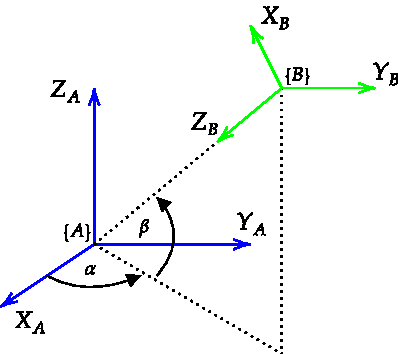
\includegraphics[scale=1]{images/robotica_tarea_2_problema_1.pdf}
    \caption{Localización del sistema ${B}$ con respecto al ${A}$}
    \label{fig:problema_1}
\end{figure}

La \autoref{fig:problema_1} muestra la localización del sistema ${B}$ con respecto al ${A}$ cuando la posición de este último viene dada por el vector $\sys{A}{{B}} = (x, y, z)^T$. La orientación de ${B}$ con respecto al ${A}$ se define de la siguiente forma:

El eje $Z_B$ apunta hacia el origen de coordenadas del sistema $\{A\}$, el eje $X_B$ avanza en el sentido positivo del eje $Z_A$, y por último, el eje $Y_B$ está contenido en un plano paralelo al formado por $X_A$ e $Y_A$.
\begin{itemize}
    \item Se pide el cálculo de la localización de $\{B\}$ con respecto al $\{A\}$, representada por la transformada homogénea $\sys{A}{B}$. Para ello, se emplea la siguiente metodología:
    \begin{itemize}
        \item Plantear los ángulos de giro a y de elevación b, que definen la orientación del sistema $\{B\}$, en función del vector de posición $\sys{A}{{B}} = (x, y, z)^T$. 
        \item Suponer un sistema móvil coincidente con $\{A\}$ y que se verá modificado a través de rotaciones y desplazamientos. 
        \item Elaborar una secuencia de transformaciones homogéneas elementales que, tras aplicarlas, consiga que este sistema móvil coincida perfectamente con $\{B\}$. 
    \end{itemize}

    \item Construir una función MATLAB que posea como argumento el vector de posición del sistema de coordenadas ${B}$, y retorne la matriz de transformación homogénea que relacione el mencionado sistema con el global de referencias $\{A\}$ y utilizarla en el caso de $\sys{A}{{B}} = (100, 70, 150)^T$. Representar ambos sistemas con \texttt{createFRAME}.
\end{itemize} 

    El \autoref{transformada_ATB} es una \textbf{función} que mediante trigonometría calcula los ángulos $\alpha$, $\beta$ y la matriz que representan los distintos giros y desplazamientos, en este caso \textit{móviles}, que consiguen el sistema $\{B\}$. La función minimiza los fallos usando el seno y coseno junto con la función \texttt{atan2} que ofrece \textit{MATLAB}.
    
    \begin{minipage}[c]{\linewidth}
    \lstinputlisting[caption={Matriz de la transformada $\sys{A}{B}$.},captionpos=b,label={transformada_ATB}, language={MATLAB}]{codes/robotica_tarea_2_code_1.m}
    \end{minipage}

    Con la función ya implementada en el \autoref{transformada_ATB} generamos el \autoref{ATB_used}, en el que definimos el punto solicitado y lo intruducimos en la función \texttt{calculate\_transformation}.

    \lstinputlisting[caption={Matriz de la transformada $\sys{A}{B}$.},captionpos=b,label={ATB_used}, language={MATLAB}]{codes/robotica_tarea_2_code_2.m}    

    Obtenemos los siguientes resultados: 
    \begin{verbatim}
        BTO =
             0     1     0    11
            -1     0     0    10
             0     0     1     1
             0     0     0     1
    \end{verbatim}


    \begin{minipage}[c]{\linewidth}
        \lstinputlisting[caption={Representación del sistema mediante las funciones del createFrame},captionpos=b,label={createframe}, language={MATLAB}]{codes/robotica_tarea_2_code_4.m}
        \end{minipage}    


    La representación de una base y del sistema hallado, mediante el \autoref{createframe},
    da el siguiente resultado:

    \begin{figure}[H]
        \centering
        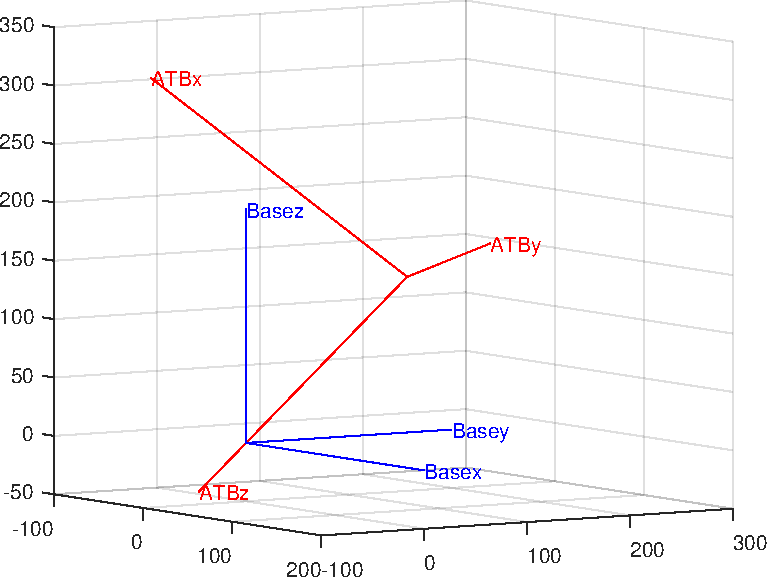
\includegraphics[scale = 1]{images/robotica_tare2_problema_1.pdf}
        \caption{Representación de los sistemas.}
        \label{representacion_createframe}
    \end{figure}

Como se puede observar en la \autoref{representacion_createframe} el eje ${}^AT_{B_{Z}}$ cumple las especificaciones, la prolongación de dicho eje corta el origen el eje ${}^AT_{B_{y}}$ está contenida en un plano paralelo a la base.
    
    \section*{Problema \# 2}

Se desea calcular la matriz de rotación que define la orientación de un sistema móvil $\{H\}$ con respecto a uno de referencias fijo $\{B\}$ definida de la siguiente forma: 

Efectuar una rotación de un ángulo $\alpha$ respecto al eje $X_B$, seguida por un giro $\beta$ respecto al eje $Z_H$ y seguida por rotación de un ángulo $\gamma$ respecto a $Y_B$.
\begin{itemize}
    \item Deducir  la  representación  en  ángulos  OAT  que  corresponde  al  enunciado  propuesto aplicando la  metodología  denominada  el problema  inverso  de  la  orientación.

    Implantarlo en MATLAB teniendo en cuenta las soluciones degeneradas.    

    \begin{minipage}[c]{\linewidth}    
    \lstinputlisting[caption={Función para obtener los valores de la representación $OAT$.},captionpos=b,label={tr2OAT}, language={MATLAB}]{codes/robotica_tarea_2_code_3.m}    
    \end{minipage}

    \begin{minipage}[c]{\linewidth}    
        \lstinputlisting[caption={Ángulos OAT},captionpos=b,label={codigo1}, language={MATLAB}]{codes/robotica_tarea_2_code_5.m}    
        \end{minipage}    

La salida del \autoref{codigo1} es la siguiente:
\begin{equation*}
    \left(\begin{array}{cccc}
        \cos \left(\beta \right)\,\cos \left(\gamma \right)+\sin \left(\alpha \right)\,\sin \left(\beta \right)\,\sin \left(\gamma \right) & \cos \left(\beta \right)\,\sin \left(\alpha \right)\,\sin \left(\gamma \right)-\cos \left(\gamma \right)\,\sin \left(\beta \right) & \cos \left(\alpha \right)\,\sin \left(\gamma \right) & 0\\
        \cos \left(\alpha \right)\,\sin \left(\beta \right) & \cos \left(\alpha \right)\,\cos \left(\beta \right) & -\sin \left(\alpha \right) & 0\\
        \cos \left(\gamma \right)\,\sin \left(\alpha \right)\,\sin \left(\beta \right)-\cos \left(\beta \right)\,\sin \left(\gamma \right) & \sin \left(\beta \right)\,\sin \left(\gamma \right)+\cos \left(\beta \right)\,\cos \left(\gamma \right)\,\sin \left(\alpha \right) & \cos \left(\alpha \right)\,\cos \left(\gamma \right) & 0\\
        0 & 0 & 0 & 1
        \end{array}\right)
\end{equation*}

    
    \begin{verbatim}
        O = 0.7137
        A = -0.3614
        T = 0.9112
        O = -2.4279
        A = -2.7802
        T = -2.2304
    \end{verbatim}  
        
         
    \item Volver  a  calcular  la  matriz  de  orientación  detallada  en  el  enunciado si  la  situación inicial entre el sistema $\{B\}$ y $\{H\}$ se define de la siguiente manera: 
    El eje $Z_H$ coincide con $X_B$, $X_H$ con $-Y_B$ e $Y_H$ con $-Z_B$. A partir de esta situación se realizarán las transformaciones dadas inicialmente.
    
    Probar la función elaborada con los siguientes datos: $\alpha=45^\circ$, $\beta=30^\circ$ y $\gamma=60^\circ$.

    \begin{minipage}[c]{\linewidth}    
        \lstinputlisting[caption={Ángulos OAT},captionpos=b,label={codigo2}, language={MATLAB}]{codes/robotica_tarea_2_code_6.m}    
        \end{minipage}    
    
    Obtenemos los siguientes resultados, la nueva matriz y los ángulos $OAT$. 

    \begin{verbatim}
     BTH_2 = 4×4    
        -0.8365   -0.2241    0.5000         0
        -0.2588    0.9659         0         0
        -0.4830   -0.1294   -0.8660         0
              0         0         0    1.0000    

     O = 1.5708
     A = 1.0472
     T = -0.2618
     O = -1.5708
     A = 2.0944
     T = 2.8798
    \end{verbatim}    
\end{itemize}
\end{document}